\chapter{Math}
\section{Thinking in Math}
\subsection{Decimal System}
The {\color{blue}{decimal system}}, also known as the {\color{blue}{base-$10$ system}}, is a {\color{blue}{positional system}} that uses the numbers $0$ through $9$ as its {\color{blue}{base}}. In this system, the value of each {\color{blue}{digit}} is determined by its position, also referred to as its {\color{blue}{place value}}.

\begin{equation}
123.45 = 1 \times 10^2 + 2 \times 10^1 + 3 \times 10^0 + 4 \times 10^{-1} + 5 \times 10^{-2}
\end{equation}

\subsection{Built-in Character Types}
C/C++ provides a variety of {\color{blue}{character types}}, and here are the most common ones:
\begin{itemize}
\item {\colorbox{CodeBackground}{\lstinline|char|}}: the default character type, which is usually {\colorbox{CodeBackground}{\lstinline|8|}}-bits.
\item {\colorbox{CodeBackground}{\lstinline|signed char|}}: Like {\colorbox{CodeBackground}{\lstinline|char|}}, but guaranteed to be {\colorbox{CodeBackground}{\lstinline|signed|}}, which means they can hold both {\color{blue}{positive}} and {\color{blue}{negative}} values. 
\item {\colorbox{CodeBackground}{\lstinline|unsigned char|}}: Like {\colorbox{CodeBackground}{\lstinline|char|}}, but guaranteed to be {\colorbox{CodeBackground}{\lstinline|unsigned|}}, which means they can only hold {\color{blue}{positive}} values.
\end{itemize}

In C++, whether the {\colorbox{CodeBackground}{\lstinline|char|}} type is {\colorbox{CodeBackground}{\lstinline|signed|}} or {\colorbox{CodeBackground}{\lstinline|unsigned|}} is {\color{blue}{implementation-defined}}. This means it is up to the compiler and the system it's compiling for. Some systems define {\colorbox{CodeBackground}{\lstinline|char|}} as {\colorbox{CodeBackground}{\lstinline|signed|}} by default, while others define it as {\colorbox{CodeBackground}{\lstinline|unsigned|}}. So, if you want to ensure portability of your code and you need a {\colorbox{CodeBackground}{\lstinline|char|}} type with a specific sign ({\colorbox{CodeBackground}{\lstinline|signed|}} or {\colorbox{CodeBackground}{\lstinline|unsigned|}}), you should explicitly use {\colorbox{CodeBackground}{\lstinline|signed char|}} or {\colorbox{CodeBackground}{\lstinline|unsigned char|}}.\\

\subsubsection*{Character Types v.s. Integer Types}
Note that {\color{blue}{character types}} are indeed {\color{blue}{integer types}}, so that {\color{blue}{arithmetic}} and {\color{blue}{bitwise logical operations}} apply. \\

The ASCII {\color{blue}{characters}} and their corresponding {\color{blue}{values}} are illustrated as follows.
\begin{figure}[H]
\centering
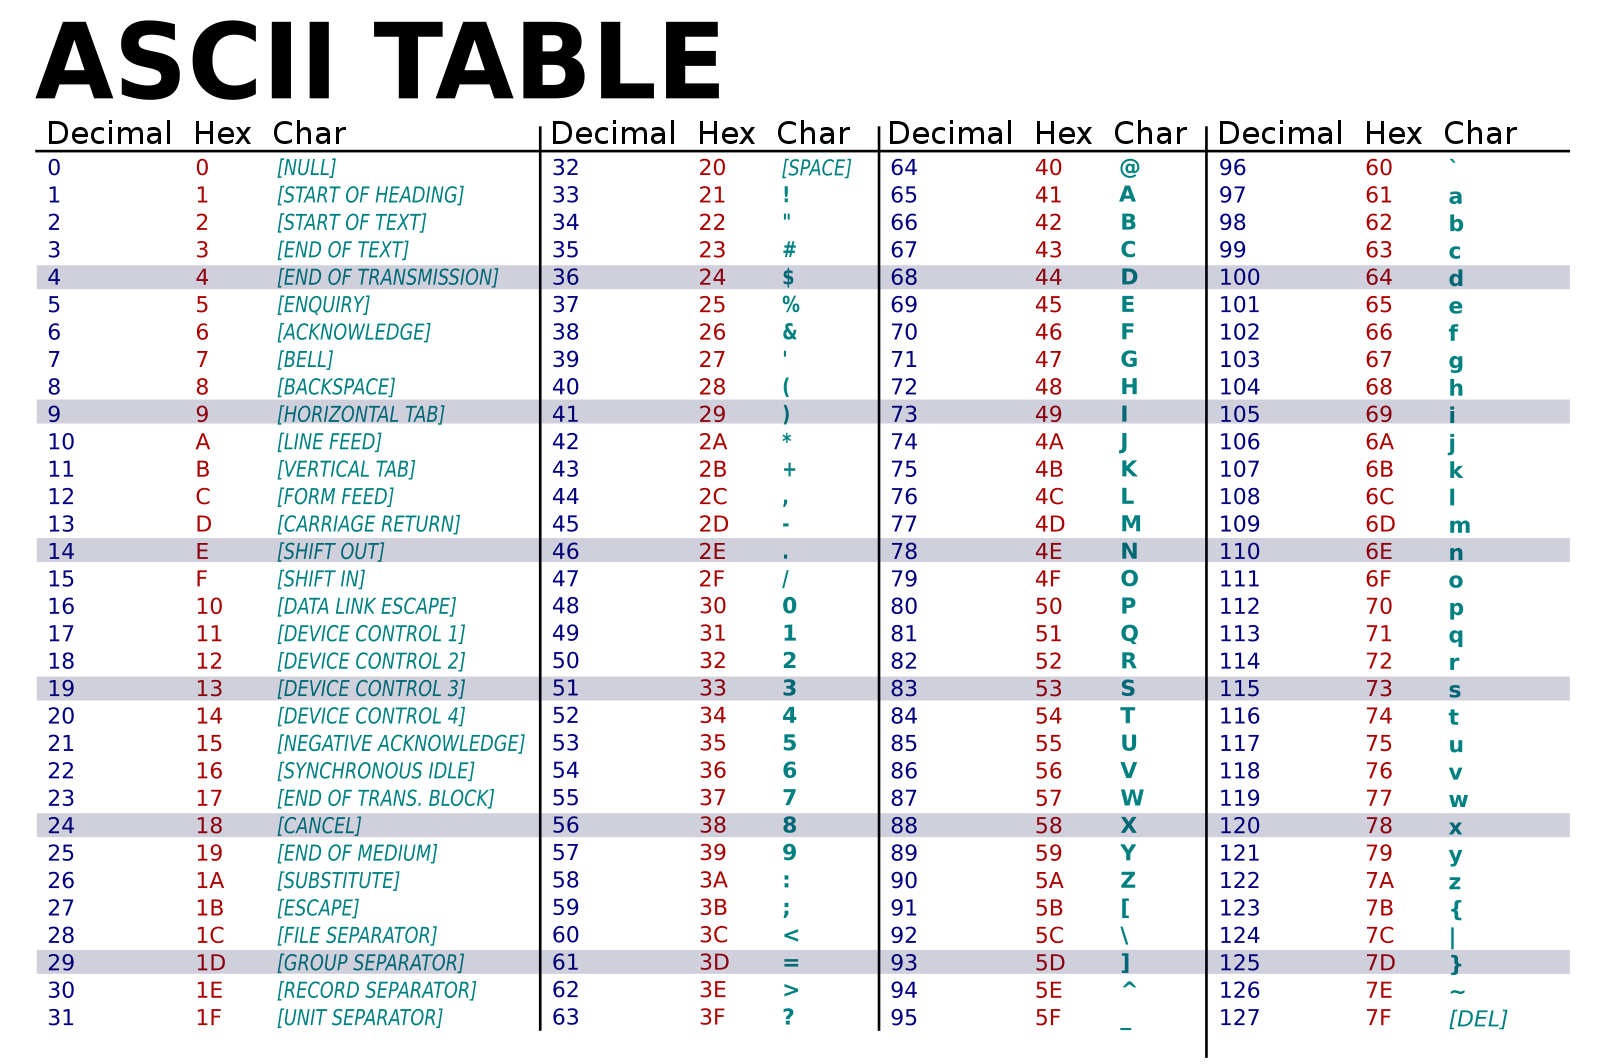
\includegraphics[width=0.8\linewidth]{images/ascii_table.svg}
\label{fig:asciitable}
\end{figure}
\subsection{Built-in Integer Types}
In C++, there are four main sizes of integer types:
\begin{itemize}
\item {\colorbox{CodeBackground}{\lstinline|short int|}}, a.k.a., {\colorbox{CodeBackground}{\lstinline|short|}};
\item "plain" {\colorbox{CodeBackground}{\lstinline|int|}};
\item {\colorbox{CodeBackground}{\lstinline|long int|}}, a.k.a., {\colorbox{CodeBackground}{\lstinline|long|}};
\item {\colorbox{CodeBackground}{\lstinline|long long int|}}, a.k.a., {\colorbox{CodeBackground}{\lstinline|long long|}}
\end{itemize}
By default, these types are {\colorbox{CodeBackground}{\lstinline|signed|}}, meaning they can represent both {\color{blue}{positive}} and {\color{blue}{negative}} values. However, you can explicitly specify them as either {\colorbox{CodeBackground}{\lstinline|signed|}} or {\colorbox{CodeBackground}{\lstinline|unsigned|}} to control whether they can hold negative values.

\subsubsection*{Integer Literals}
We only talk about {\color{blue}{decimal integer literals}} here.

\begin{itemize}
\item no suffix $\rightarrow$ {\colorbox{CodeBackground}{\lstinline|int|}}, {\colorbox{CodeBackground}{\lstinline|long int|}}, or {\colorbox{CodeBackground}{\lstinline|long long int|}}
\item suffixed by {\colorbox{CodeBackground}{\lstinline|u|}} or {\colorbox{CodeBackground}{\lstinline|U|}} $\rightarrow$ {\colorbox{CodeBackground}{\lstinline|unsigned int|}}, {\colorbox{CodeBackground}{\lstinline|unsigned long int|}}, or {\colorbox{CodeBackground}{\lstinline|unsigned long long int|}}
\item suffixed by {\colorbox{CodeBackground}{\lstinline|l|}} or {\colorbox{CodeBackground}{\lstinline|L|}} $\rightarrow$ {\colorbox{CodeBackground}{\lstinline|long int|}}, {\colorbox{CodeBackground}{\lstinline|long long int|}}
\item suffixed by {\colorbox{CodeBackground}{\lstinline|ul|}}, {\colorbox{CodeBackground}{\lstinline|lu|}}, {\colorbox{CodeBackground}{\lstinline|uL|}}, {\colorbox{CodeBackground}{\lstinline|Lu|}}, {\colorbox{CodeBackground}{\lstinline|Ul|}}, {\colorbox{CodeBackground}{\lstinline|lU|}}, {\colorbox{CodeBackground}{\lstinline|UL|}}, or {\colorbox{CodeBackground}{\lstinline|LU|}} $\rightarrow$ {\colorbox{CodeBackground}{\lstinline|unsigned long int|}} or {\colorbox{CodeBackground}{\lstinline|unsigned long long int|}}
\item suffixed by {\colorbox{CodeBackground}{\lstinline|ll|}} or {\colorbox{CodeBackground}{\lstinline|LL|}} $\rightarrow$ {\colorbox{CodeBackground}{\lstinline|long long int|}}
\item suffixed by {\colorbox{CodeBackground}{\lstinline|llu|}}, {\colorbox{CodeBackground}{\lstinline|llU|}}, {\colorbox{CodeBackground}{\lstinline|ull|}}, {\colorbox{CodeBackground}{\lstinline|Ull|}}, {\colorbox{CodeBackground}{\lstinline|LLu|}}, {\colorbox{CodeBackground}{\lstinline|LLU|}}, {\colorbox{CodeBackground}{\lstinline|uLL|}}, or {\colorbox{CodeBackground}{\lstinline|ULL|}} $\rightarrow$ {\colorbox{CodeBackground}{\lstinline|unsigned long long int|}}
\end{itemize}

\subsection{Built-in Floating Point Types}
There are three floating-point types in C++:
\begin{itemize}
\item {\colorbox{CodeBackground}{\lstinline|float|}} (single-precision);
\item {\colorbox{CodeBackground}{\lstinline|double|}} (double-precision);
\item {\colorbox{CodeBackground}{\lstinline|long double|}} (extended-precision);
\end{itemize}

\subsubsection*{Floating Point Literals}
\begin{itemize}
\item By default, a floating-point literal is of type {\colorbox{CodeBackground}{\lstinline|double|}}.
\item If you want a floating-point literal of type {\colorbox{CodeBackground}{\lstinline|float|}}, you can define one using the suffix {\colorbox{CodeBackground}{\lstinline|f|}} or {\colorbox{CodeBackground}{\lstinline|F|}}.
\item If you want a floating-point literal of type {\colorbox{CodeBackground}{\lstinline|long double|}}, you can define one using the suffix {\colorbox{CodeBackground}{\lstinline|l|}} or {\colorbox{CodeBackground}{\lstinline|L|}}.
\end{itemize}

\section{LC 0002 - Add Two Numbers Represented in Linked List}\label{lc0002}
You are given two \ul{non-empty} \ul{singly linked lists} representing two \ul{non-negative} integers. \\

The digits are stored in \ul{reverse order}, which means the digits are ordered from \ul{least significant} to \ul{most significant} in \ul{left-to-right order}. \\

Add the two numbers and return the sum as a singly linked list.\\

You may assume the two numbers do not contain any \ul{leading zero}, except the number {\colorbox{CodeBackground}{\lstinline|0|}} itself.\\

Examples: 
\begin{itemize}
	\item {\colorbox{CodeBackground}{\lstinline|[2 -> 4 -> 3] + [5 -> 6 -> 5] --> [7 -> 0 -> 8]|}}
\end{itemize}

\subsection*{Solution}
\begin{lstlisting}
ListNode* addTwoNumbers(ListNode* l1, ListNode* l2) {
  ListNode* dummy_head = new ListNode();
  ListNode* cur_digit = dummy_head;
  int carry = 0;
  while (l1 || l2 || carry) {
    int sum = carry;
    if (l1) {
      sum += l1->val;
      l1 = l1->next;
    }
    if (l2) {
      sum += l2->val;
      l2 = l2->next;
    }
    cur_digit->next = new ListNode(sum % 10);
    cur_digit = cur_digit->next;
    carry = sum / 10;
  }
  return dummy_head->next;
}
\end{lstlisting}

\subsection*{Related - ADD}
\begin{itemize}
\item \hyperref[lc0002]{LC 0002 - Add Two Numbers Represented in Linked List}
\item \hyperref[lc0415]{LC 0415 - Add Two Numbers Represented in Strings}
\item \hyperref[lc0067]{LC 0067 - Add Two Binary Numbers Represented in String}
\item \hyperref[lc0066]{LC 0066 - Plus One}
\end{itemize}

\section{LC 0415 - Add Two Numbers Represented in Strings}\label{lc0415}
Given two \ul{non-negative} integers, {\colorbox{CodeBackground}{\lstinline|num1|}} and {\colorbox{CodeBackground}{\lstinline|num2|}} represented as string (both {\colorbox{CodeBackground}{\lstinline|nums1|}} and {\colorbox{CodeBackground}{\lstinline|nums2|}} are \ul{non-empty}), return the sum of {\colorbox{CodeBackground}{\lstinline|num1|}} and {\colorbox{CodeBackground}{\lstinline|num2|}} as a string.\\

Examples:
\begin{itemize}
\item {\colorbox{CodeBackground}{\lstinline|num1 = "11", num2 = "123" --> "134"|}}
\item {\colorbox{CodeBackground}{\lstinline|num1 = "456", num2 = "77" --> "533"|}}
\item {\colorbox{CodeBackground}{\lstinline|num1 = "0", num2 = "0" --> "0"|}}
\end{itemize}

\subsection*{Solution}
\begin{lstlisting}
std::string addStrings(std::string num1, std::string num2) {
  std::string sum_str;
  int carry = 0;
  int i = num1.size() - 1;
  int j = num2.size() - 1;
  while (i >= 0 || j >= 0 || carry) {
    int sum = carry;
    if (i >= 0) {
      sum += num1[i] - '0';
      --i;
    }
    if (j >= 0) {
      sum += num2[j] - '0';
      --j;
    }
    sum_str.push_back(sum % 10 + '0');
    carry = sum / 10;
  }
  std::reverse(sum_str.begin(), sum_str.end());
  return sum_str;
}
\end{lstlisting}

\subsection*{Related - ADD}
\begin{itemize}
\item \hyperref[lc0002]{LC 0002 - Add Two Numbers Represented in Linked List}
\item \hyperref[lc0415]{LC 0415 - Add Two Numbers Represented in Strings}
\item \hyperref[lc0067]{LC 0067 - Add Two Binary Numbers Represented in String}
\item \hyperref[lc0066]{LC 0066 - Plus One}
\end{itemize}

\subsection*{Related - String + Basic Mathematical Operation}
\begin{itemize}
\item \hyperref[lc0415]{LC 0415 - Add Two Numbers Represented in Strings}
\item \hyperref[lc0043]{LC 0043 - Multiply Strings}
\end{itemize}

\section{LC 0067 - Add Two Binary Numbers Represented in String}\label{lc0067}
Given two \ul{non-empty} binary strings {\colorbox{CodeBackground}{\lstinline|a|}} and {\colorbox{CodeBackground}{\lstinline|b|}}, return their sum as a binary string.\\

Examples:
\begin{itemize}
	\item {\colorbox{CodeBackground}{\lstinline|a = "11", b = "1" --> "100"|}}
	\item {\colorbox{CodeBackground}{\lstinline|a = "1010", b = "1011" --> "10101"|}}
\end{itemize}

\subsection*{Solution}
\begin{lstlisting}
std::string addBinary(std::string a, std::string b) {
  std::string sum_str = "";
  int i = a.size() - 1;
  int j = b.size() - 1;
  int carry = 0;
  while (i >= 0 || j >= 0 || carry) {
    int sum = carry;
    if (i >= 0) {
      sum += a[i] - '0';
      --i;
    }
    if (j >= 0) {
      sum += b[j] - '0';
      --j;
    }
    sum_str.push_back((sum % 2) + '0');
    carry = sum / 2;
  }
  std::reverse(sum_str.begin(), sum_str.end());
  return sum_str;
}
\end{lstlisting}

\subsection*{Related - ADD}
\begin{itemize}
\item \hyperref[lc0002]{LC 0002 - Add Two Numbers Represented in Linked List}
\item \hyperref[lc0415]{LC 0415 - Add Two Numbers Represented in Strings}
\item \hyperref[lc0067]{LC 0067 - Add Two Binary Numbers Represented in String}
\item \hyperref[lc0066]{LC 0066 - Plus One}
\end{itemize}

\section{LC 0066 - Plus One}\label{lc0066}
You are given a \ul{large integer} represented as a \ul{non-empty} \ul{integer array} {\colorbox{CodeBackground}{\lstinline|digits|}}, where each {\colorbox{CodeBackground}{\lstinline|digits[i]|}} is the {\colorbox{CodeBackground}{\lstinline|i|}}th digit of the integer. \\

The digits are ordered from \ul{most significant} to \ul{least significant} in \ul{left-to-right order}. \\

Increment the large integer by one and return the resulting array of digits.\\

You may assume the two numbers do not contain any \ul{leading zero}, except the number {\colorbox{CodeBackground}{\lstinline|0|}} itself.\\

Examples:
\begin{itemize}
\item {\colorbox{CodeBackground}{\lstinline|digits = [1,2,3] --> [1,2,4]|}}
\item {\colorbox{CodeBackground}{\lstinline|digits = [4,3,2,1] --> [4,3,2,2]|}}
\item {\colorbox{CodeBackground}{\lstinline|digits = [9] --> [1,0]|}}
\end{itemize}

\subsection*{Solution}
\begin{lstlisting}
std::vector<int> plusOne(std::vector<int>& digits) {
  for (int i = digits.size() - 1; i >= 0; --i) {
    if (digits[i] < 9) {
      ++digits[i];
      return digits;
    }
    digits[i] = 0;
  }
  digits.insert(digits.begin(), 1);
  return digits;
}
\end{lstlisting}

\subsection*{Related - ADD}
\begin{itemize}
\item \hyperref[lc0002]{LC 0002 - Add Two Numbers Represented in Linked List}
\item \hyperref[lc0415]{LC 0415 - Add Two Numbers Represented in Strings}
\item \hyperref[lc0067]{LC 0067 - Add Two Binary Numbers Represented in String}
\item \hyperref[lc0066]{LC 0066 - Plus One}
\end{itemize}

\section{LC 0043 - Multiply Strings}\label{lc0043}
You are given two \ul{non-empty} \ul{non-negative} integers {\colorbox{CodeBackground}{\lstinline|num1|}} and {\colorbox{CodeBackground}{\lstinline|num2|}} represented as \ul{strings}. \\

The digits are ordered from \ul{most significant} to \ul{least significant} in \ul{left-to-right order}. \\

Return the product of {\colorbox{CodeBackground}{\lstinline|num1|}} and {\colorbox{CodeBackground}{\lstinline|num2|}}, also represented as a string.\\

Note: 
\begin{itemize}
\item Strings {\colorbox{CodeBackground}{\lstinline|num1|}} and {\colorbox{CodeBackground}{\lstinline|num2|}} consist of digits only.
\item {\colorbox{CodeBackground}{\lstinline|num1|}} and {\colorbox{CodeBackground}{\lstinline|num2|}} do not contain any \ul{leading zero}, except the number {\colorbox{CodeBackground}{\lstinline|0|}} itself.
\end{itemize}\mbox{}

Examples:
\begin{itemize}
\item {\colorbox{CodeBackground}{\lstinline|num1 = "2", num2 = "3" --> "6"|}}
\item {\colorbox{CodeBackground}{\lstinline|num1 = "123", num2 = "456" --> "56088"|}}
\end{itemize}

\subsection*{Solution}
\begin{lstlisting}
std::string multiply(std::string num1, std::string num2) {
  if (num1 == "0" || num2 == "0") { return "0"; }
  int n1 = num1.size();
  int n2 = num2.size();
  std::vector<int> res_vec(n1 + n2, 0);
  for (int i = n1 - 1; i >= 0; --i) {
    for (int j = n2 - 1; j >= 0; --j) {
      int mul = res_vec[i + j + 1] + (num1[i] - '0') * (num2[j] - '0');
      res_vec[i + j + 1] = mul % 10;
      res_vec[i + j] += mul / 10;
    }
  }
  std::string res_str;
  int i = 0;
  while (i < res_vec.size() && res_vec[i] == 0) { ++i; }
  while (i < res_vec.size()) {
    res_str.push_back(res_vec[i] + '0');
    ++i;
  }
  return res_str;
}
\end{lstlisting}

\subsection*{Related - String + Basic Mathematical Operation}
\begin{itemize}
\item \hyperref[lc0415]{LC 0415 - Add Two Numbers Represented in Strings}
\item \hyperref[lc0043]{LC 0043 - Multiply Strings}
\end{itemize}

\section{LC 0029 - Divide Two Integers}
Given two integers {\colorbox{CodeBackground}{\lstinline|dividend|}} and {\colorbox{CodeBackground}{\lstinline|divisor|}} ({\colorbox{CodeBackground}{\lstinline|divisor != 0|}}), divide two integers without using \ul{multiplication}, \ul{division}, and \ul{mod} operator.\\

The integer division should \ul{truncate toward zero}, which means losing its \ul{fractional part}. For example, {\colorbox{CodeBackground}{\lstinline|8.345|}} would be truncated to {\colorbox{CodeBackground}{\lstinline|8|}}, and {\colorbox{CodeBackground}{\lstinline|-2.7335|}} would be truncated to {\colorbox{CodeBackground}{\lstinline|-2|}}.\\

Return the \ul{quotient} after dividing {\colorbox{CodeBackground}{\lstinline|dividend|}} by {\colorbox{CodeBackground}{\lstinline|divisor|}}.\\

Note: Assume we are dealing with an environment that could only store integers within the {\colorbox{CodeBackground}{\lstinline|32|}}-bit signed integer range:  {\colorbox{CodeBackground}{\lstinline|[-2^31, 2^31 - 1]|}}.  For this problem, if the quotient is strictly greater than {\colorbox{CodeBackground}{\lstinline|2^31 - 1|}}, then return {\colorbox{CodeBackground}{\lstinline|2^31 - 1,|}} and if the quotient is strictly less than {\colorbox{CodeBackground}{\lstinline|-2^31|}}, then return {\colorbox{CodeBackground}{\lstinline|-2^31|}}.

\subsection*{*Solution - Repeated Subtraction (Time Limit Exceeded)}\label{solution:lc0029_repeated_substraction}
\begin{lstlisting}
int divide(int dividend, int divisor) {
  // edge case - overflow
  if (dividend == std::numeric_limits<int>::min() && divisor == -1) {
    return std::numeric_limits<int>::max();
  }
  int sign = ((dividend < 0) ^ (divisor < 0)) ? -1 : 1;
  // use long type to avoid overflow
  long cur_dividend = std::abs(static_cast<long>(dividend));
  long cur_divisor = std::abs(static_cast<long>(divisor));
  long quotient = 0;
  while (cur_dividend >= cur_divisor) {
    cur_dividend -= cur_divisor;
    quotient++;
  }
  return sign * quotient;
}
\end{lstlisting}

\subsection*{Other Solutions}
\begin{itemize}
%\item \hyperref[solution:lc0029_repeated_substraction]{*Repeated Subtraction (Time Limit Exceeded)}
\item \hyperref[solution:lc0029_bit_manipulation]{Bit Manipulation}
\end{itemize}

\section{LC 0166 - Fraction to Recurring Decimal}
Given two integers representing the {\colorbox{CodeBackground}{\lstinline|numerator|}} and {\colorbox{CodeBackground}{\lstinline|denominator|}} ({\colorbox{CodeBackground}{\lstinline|denominator != 0|}}) of a \ul{fraction}, return the fraction in string format.\\

If the fractional part is repeating, enclose the repeating part in parentheses.\\

If multiple answers are possible, return any of them.\\

Note that {\colorbox{CodeBackground}{\lstinline|denominator != 0|}}.\\

Examples:
\begin{itemize}
\item {\colorbox{CodeBackground}{\lstinline|numerator = 1, denominator = 2 --> "0.5"|}}
\item {\colorbox{CodeBackground}{\lstinline|numerator = 2, denominator = 1 --> "2"|}}
\item {\colorbox{CodeBackground}{\lstinline|numerator = 4, denominator = 333 --> "0.(012)"|}}
\end{itemize}

\subsection*{Solution}
\begin{lstlisting}
std::string fractionToDecimal(int numerator, int denominator) {
  if (numerator == 0) { return "0"; }
  std::string res_str;
  // sign
  if (numerator < 0 ^ denominator < 0) { res_str += '-'; }
  // integral part
  long n = std::abs(numerator);
  long d = std::abs(denominator);
  long quotient = n / d;
  res_str += std::to_string(quotient);
  long remainder = n % d;
  if (remainder == 0) { return res_str; }
  res_str += '.';
  // fractional part
  std::unordered_map<long, int> remainder2pos;
  while (remainder != 0) {
    if (remainder2pos.find(remainder) != remainder2pos.end()) {
      res_str.insert(remainder2pos[remainder], "(");
      res_str += ')';
      break;
    }
    remainder2pos[remainder] = res_str.size();
    remainder *= 10;
    quotient = remainder / d;
    res_str += std::to_string(quotient);
    remainder = remainder % d;
  }
  return res_str;
}
\end{lstlisting}

\section{LC 0367 - Valid Perfect Square}\label{lc0367}
Given an integer {\colorbox{CodeBackground}{\lstinline|num|}} ({\colorbox{CodeBackground}{\lstinline|num >= 1|}}), return {\colorbox{CodeBackground}{\lstinline|true|}} if {\colorbox{CodeBackground}{\lstinline|num|}} is a \ul{perfect square} or {\colorbox{CodeBackground}{\lstinline|false|}} otherwise.\\

A \ul{perfect square} is an integer that is the square of an integer.\\

Examples:
\begin{itemize}
\item {\colorbox{CodeBackground}{\lstinline|num = 16 --> true|}}
\item {\colorbox{CodeBackground}{\lstinline|num = 14 --> false|}}
\end{itemize}

\subsection*{Solution - Binary Search}
\begin{lstlisting}
bool isPerfectSquare(int num) {
  if (num < 2) { return true; }
  long left = 2;
  long right = num / 2;
  while (left <= right) {
    long mid = left + (right - left) / 2;
    long guess = mid * mid;
    if (guess == num) { return true; }
    if (guess < num) {
      left = mid + 1;
    } else {
      right = mid - 1;
    }
  }
  return false;
}
\end{lstlisting}

\subsection*{Related - Square Number}
\begin{itemize}
\item \hyperref[lc0367]{LC 0367 - Valid Perfect Square}
\item \hyperref[lc0279]{LC 0279 - Perfect Squares}
\end{itemize}

\section{LC 0069 - Sqrt(x)}
Given a \ul{non-negative} integer {\colorbox{CodeBackground}{\lstinline|x|}}, return the \ul{square root} of {\colorbox{CodeBackground}{\lstinline|x|}} \ul{rounded down to the nearest integer}. The returned integer should be non-negative as well.\\

Examples:
\begin{itemize}
\item {\colorbox{CodeBackground}{\lstinline|x = 4 --> 2|}}
\item {\colorbox{CodeBackground}{\lstinline|x = 8 --> 2|}}
\end{itemize}

\subsection*{Solution - Binary Search}
\begin{lstlisting}
int mySqrt(int x) {
  if (x < 2) { return x; }
  long left = 1;
  long right = x / 2;
  while (left <= right) {
    long mid = left + (right - left) / 2;
    long sq = mid * mid;
    if (sq == x) {
      return mid;
    } else if (sq < x) {
      left = mid + 1;
    } else {
      right = mid - 1;
    }
  }
  return right;
}
\end{lstlisting}

\section{LC 0050 - Pow(x, n)}
Implement {\colorbox{CodeBackground}{\lstinline|pow(x, n)|}}, which calculates {\colorbox{CodeBackground}{\lstinline|x|}} raised to the power {\colorbox{CodeBackground}{\lstinline|n|}} (i.e., $x^n$).\\

Note that either {\colorbox{CodeBackground}{\lstinline|x != 0|}} or {\colorbox{CodeBackground}{\lstinline|n > 0|}}.\\

Examples:
\begin{itemize}
\item {\colorbox{CodeBackground}{\lstinline|x = 2.00000, n = 10 --> 1024.00000|}}
\item {\colorbox{CodeBackground}{\lstinline|x = 2.10000, n = 3 --> 9.26100|}}
\item {\colorbox{CodeBackground}{\lstinline|x = 2.00000, n = -2 --> 0.25000|}}
\end{itemize}


\subsection*{Solution 1 - Without Casting}
\begin{lstlisting}
double myPow(double x, int n) {
  // n is negative
  if (n < 0) {
    x = 1 / x;
    // avoid overflow when n is std::numeric_limits<int>::min().
    n = -(n + 1);
    return x * PosPow(x, n);
  }
  // n is positive
  return PosPow(x, n);
}

double PosPow(double x, int n) {
  // base case - power 0
  if (n == 0) { return 1.0; }
  double half = PosPow(x, n / 2);
  if (n % 2 == 0) {
    return half * half;
  } else {
    return half * half * x;
  }
}
\end{lstlisting}

\subsection*{Solution 2 - With Casting}
\begin{lstlisting}
double myPow(double x, int n) {
  // n is negative
  if (n < 0) {
    x = 1 / x;
    long ln = -1 * static_cast<long>(n);
    return PosPow(x, n);
  }
  // n is positive
  return PosPow(x, n);
}

double PosPow(double x, long n) {
  // base case - power 0
  if (n == 0) { return 1.0; }
  double half = PosPow(x, n / 2);
  if (n % 2 == 0) {
    return half * half;
  } else {
    return half * half * x;
  }
}
\end{lstlisting}

\section{LC 0231 - Power of Two}
Given an integer {\colorbox{CodeBackground}{\lstinline|n|}}, return {\colorbox{CodeBackground}{\lstinline|true|}} if it is a power of {\colorbox{CodeBackground}{\lstinline|2|}}. Otherwise, return {\colorbox{CodeBackground}{\lstinline|false|}}.\\

Examples:
\begin{itemize}
\item {\colorbox{CodeBackground}{\lstinline|n = 1 -> true|}}
\item {\colorbox{CodeBackground}{\lstinline|n = 16 --> true|}}
\item {\colorbox{CodeBackground}{\lstinline|n = 3 --> false|}}
\end{itemize}

\subsection*{Solution - Simulation (Iterative)}\label{solution:lc0231_simulation_iterative}
\begin{lstlisting}
bool isPowerOfTwo(int n) {
  if (n <= 0) { return false; }
  while (n % 2 == 0) { n /= 2; }
  return n == 1;
}
\end{lstlisting}

\subsection*{Other Solutions}
\begin{itemize}
%\item \hyperref[solution:lc0231_simulation_iterative]{Simulation (Iterative)}
\item \hyperref[solution:lc0231_simulation_recursion]{Simulation (Recursion)}
\item \hyperref[solution:lc0231_bit_manipulation]{Bit Manipulation}
\end{itemize}

\subsection*{Related}
\begin{itemize}
\item \hyperref[lc0231]{LC 0231 - Power of Two}
\item \hyperref[lc0342]{LC 0342 - Power of Four}
\end{itemize}

\section{LC 0342 - Power of Four}
Given an integer {\colorbox{CodeBackground}{\lstinline|n|}}, return {\colorbox{CodeBackground}{\lstinline|true|}} if it is a power of {\colorbox{CodeBackground}{\lstinline|4|}}. Otherwise, return {\colorbox{CodeBackground}{\lstinline|false|}}.\\

Examples:
\begin{itemize}
\item {\colorbox{CodeBackground}{\lstinline|n = 16 --> true|}}
\item {\colorbox{CodeBackground}{\lstinline|n = 5 --> false|}}
\item {\colorbox{CodeBackground}{\lstinline|n = 1 --> true|}}
\end{itemize}

\subsection*{Solution - Iterative}\label{solution:lc0342_simulation_iterative}
\begin{lstlisting}
bool isPowerOfFour(int n) {
  if (n <= 0) { return false; }
  while (n % 4 == 0) { n /= 4; }
  return n == 1;
}
\end{lstlisting}

\subsection*{Other Solutions}
\begin{itemize}
%\item \hyperref[solution:lc0342_simulation_iterative]{Simulation (Iterative)}
\item \hyperref[solution:lc0342_simulation_recursion]{Simulation (Recursion)}
\item \hyperref[solution:lc0342_bit_manipulation]{Bit Manipulation}
\end{itemize}

\subsection*{Related}
\begin{itemize}
\item \hyperref[lc0231]{LC 0231 - Power of Two}
\item \hyperref[lc0342]{LC 0342 - Power of Four}
\end{itemize}

\section{LC 0504 - Base 7}\label{lc0504}
Given an integer {\colorbox{CodeBackground}{\lstinline|num|}}, return a string of its base {\colorbox{CodeBackground}{\lstinline|7|}} representation.\\

Examples:
\begin{itemize}
\item {\colorbox{CodeBackground}{\lstinline|num = 100 --> "202"|}}
\item {\colorbox{CodeBackground}{\lstinline|num = -7 --> "-10"|}}
\end{itemize}

\subsection*{Solution}
\begin{lstlisting}
std::string convertToBase7(int num) {
  // edge case
  if (num == 0) { return "0"; }
  std::string base7;
  bool is_negative = num < 0;
  num = std::abs(num);
  while (num > 0) {
    base7.push_back('0' + (num % 7));
    num /= 7;
  }
  if (is_negative) { base7.push_back('-'); }
  std::reverse(base7.begin(), base7.end());
  return base7;
}
\end{lstlisting}

\subsection*{Related}
\begin{itemize}
\item \hyperref[lc0504]{LC 0504 - Base 7}
\item \hyperref[lc0405]{LC 0405 - Convert a Number to Hexadecimal}
\end{itemize}

\section{LC 0013 - Roman to Integer}
\ul{Roman numerals} are represented by seven different symbols: {\colorbox{CodeBackground}{\lstinline|I|}}, {\colorbox{CodeBackground}{\lstinline|V|}}, {\colorbox{CodeBackground}{\lstinline|X|}}, {\colorbox{CodeBackground}{\lstinline|L|}}, {\colorbox{CodeBackground}{\lstinline|C|}}, {\colorbox{CodeBackground}{\lstinline|D|}} and {\colorbox{CodeBackground}{\lstinline|M|}}. The map between symbols and values are illustrated as follows.

\begin{table}[H]
\centering
\begin{tabular}{|c|c|}
\hline
Symbol & Value \\ \hline
I      & 1     \\ \hline
V      & 5     \\ \hline
X      & 10    \\ \hline
L       & 50 \\ \hline
C       & 100 \\ \hline
D       & 500 \\ \hline
M       & 1000 \\ \hline
\end{tabular}
\end{table}

For example:
\begin{itemize}
\item {\colorbox{CodeBackground}{\lstinline|2|}} is written as {\colorbox{CodeBackground}{\lstinline|II|}} in Roman numeral, just two ones added together;
\item {\colorbox{CodeBackground}{\lstinline|12|}} is written as {\colorbox{CodeBackground}{\lstinline|XII|}}, which is simply {\colorbox{CodeBackground}{\lstinline|X + II|}};
\item The number {\colorbox{CodeBackground}{\lstinline|27|}} is written as {\colorbox{CodeBackground}{\lstinline|XXVII|}}, which is {\colorbox{CodeBackground}{\lstinline|XX + V + II|}}.
\end{itemize}\mbox{}

Roman numerals are usually written \ul{largest to smallest} from \ul{left to right}. However, the numeral for \ul{four} is not {\colorbox{CodeBackground}{\lstinline|IIII|}}. Instead, the number \ul{four} is written as {\colorbox{CodeBackground}{\lstinline|IV|}}. Because the \ul{one} is before the \ul{five} we subtract it making \ul{four}. The same principle applies to the number \ul{nine}, which is written as {\colorbox{CodeBackground}{\lstinline|IX|}}. There are six instances where subtraction is used:
\begin{itemize}
\item {\colorbox{CodeBackground}{\lstinline|I|}} can be placed before {\colorbox{CodeBackground}{\lstinline|V|}} ({\colorbox{CodeBackground}{\lstinline|5|}}) and {\colorbox{CodeBackground}{\lstinline|X|}} ({\colorbox{CodeBackground}{\lstinline|10|}}) to make {\colorbox{CodeBackground}{\lstinline|4|}} and {\colorbox{CodeBackground}{\lstinline|9|}}. 
\item {\colorbox{CodeBackground}{\lstinline|X|}} can be placed before {\colorbox{CodeBackground}{\lstinline|L|}} ({\colorbox{CodeBackground}{\lstinline|50|}}) and {\colorbox{CodeBackground}{\lstinline|C|}} ({\colorbox{CodeBackground}{\lstinline|100|}}) to make {\colorbox{CodeBackground}{\lstinline|40|}} and {\colorbox{CodeBackground}{\lstinline|90|}}. 
\item {\colorbox{CodeBackground}{\lstinline|C|}} can be placed before {\colorbox{CodeBackground}{\lstinline|D|}} ({\colorbox{CodeBackground}{\lstinline|500|}}) and {\colorbox{CodeBackground}{\lstinline|M|}} ({\colorbox{CodeBackground}{\lstinline|1000|}}) to make {\colorbox{CodeBackground}{\lstinline|400|}} and {\colorbox{CodeBackground}{\lstinline|900|}}.
\end{itemize}

Given a \ul{non-empty} roman numeral {\colorbox{CodeBackground}{\lstinline|s|}}, convert it to an integer.\\

It is guaranteed that {\colorbox{CodeBackground}{\lstinline|s|}} is a valid roman numeral in the range {\colorbox{CodeBackground}{\lstinline|[1, 3999]|}}.\\

Examples:
\begin{itemize}
\item {\colorbox{CodeBackground}{\lstinline|s = "III" --> 3 (III = 3)|}}
\item {\colorbox{CodeBackground}{\lstinline|s = "LVIII" --> 58 (L = 50, V= 5, III = 3)|}}
\item {\colorbox{CodeBackground}{\lstinline|s = "MCMXCIV" --> 1994 (M = 1000, CM = 900, XC = 90 and IV = 4)|}}
\end{itemize}

\subsection*{Solution 1}
\begin{lstlisting}
int romanToInt(std::string s) {
  std::unordered_map<char, int> symbol2val = {{'I', 1},   {'V', 5},   {'X', 10},  {'L', 50},
                                              {'C', 100}, {'D', 500}, {'M', 1000}};
  int num = symbol2val[s.back()];
  for (int i = s.size() - 2; i >= 0; --i) {
    if (symbol2val[s[i]] < symbol2val[s[i + 1]]) {
      num -= symbol2val[s[i]];
    } else {
      num += symbol2val[s[i]];
    }
  }
  return num;
}
\end{lstlisting}

\subsection*{*Solution 2}
\begin{lstlisting}
int romanToInt(std::string s) {
  std::unordered_map<std::string, int> symbol2val = {
      {"I", 1},   {"IV", 4},  {"V", 5},    {"IX", 9},  {"X", 10},   {"XL", 40}, {"L", 50},
      {"XC", 90}, {"C", 100}, {"CD", 400}, {"D", 500}, {"CM", 900}, {"M", 1000}};
  int num = 0;
  for (int i = 0; i < s.size(); ++i) {
    if (i < s.size() - 1 && symbol2val.find(s.substr(i, 2)) != symbol2val.end()) {
      num += symbol2val[s.substr(i, 2)];
      ++i;
    } else {
      num += symbol2val[s.substr(i, 1)];
    }
  }
  return num;
}
\end{lstlisting}

\section{LC 0012 - Integer to Roman}
\ul{Roman numerals} are represented by seven different symbols: {\colorbox{CodeBackground}{\lstinline|I|}}, {\colorbox{CodeBackground}{\lstinline|V|}}, {\colorbox{CodeBackground}{\lstinline|X|}}, {\colorbox{CodeBackground}{\lstinline|L|}}, {\colorbox{CodeBackground}{\lstinline|C|}}, {\colorbox{CodeBackground}{\lstinline|D|}} and {\colorbox{CodeBackground}{\lstinline|M|}}. The map between symbols and values are illustrated as follows.

\begin{table}[H]
\centering
\begin{tabular}{|c|c|}
\hline
Symbol & Value \\ \hline
I      & 1     \\ \hline
V      & 5     \\ \hline
X      & 10    \\ \hline
L       & 50 \\ \hline
C       & 100 \\ \hline
D       & 500 \\ \hline
M       & 1000 \\ \hline
\end{tabular}
\end{table}

For example:
\begin{itemize}
\item {\colorbox{CodeBackground}{\lstinline|2|}} is written as {\colorbox{CodeBackground}{\lstinline|II|}} in Roman numeral, just two ones added together;
\item {\colorbox{CodeBackground}{\lstinline|12|}} is written as {\colorbox{CodeBackground}{\lstinline|XII|}}, which is simply {\colorbox{CodeBackground}{\lstinline|X + II|}};
\item The number {\colorbox{CodeBackground}{\lstinline|27|}} is written as {\colorbox{CodeBackground}{\lstinline|XXVII|}}, which is {\colorbox{CodeBackground}{\lstinline|XX + V + II|}}.
\end{itemize}\mbox{}

Roman numerals are usually written \ul{largest to smallest} from \ul{left to right}. However, the numeral for \ul{four} is not {\colorbox{CodeBackground}{\lstinline|IIII|}}. Instead, the number \ul{four} is written as {\colorbox{CodeBackground}{\lstinline|IV|}}. Because the \ul{one} is before the \ul{five} we subtract it making \ul{four}. The same principle applies to the number \ul{nine}, which is written as {\colorbox{CodeBackground}{\lstinline|IX|}}. There are six instances where subtraction is used:
\begin{itemize}
\item {\colorbox{CodeBackground}{\lstinline|I|}} can be placed before {\colorbox{CodeBackground}{\lstinline|V|}} ({\colorbox{CodeBackground}{\lstinline|5|}}) and {\colorbox{CodeBackground}{\lstinline|X|}} ({\colorbox{CodeBackground}{\lstinline|10|}}) to make {\colorbox{CodeBackground}{\lstinline|4|}} and {\colorbox{CodeBackground}{\lstinline|9|}}. 
\item {\colorbox{CodeBackground}{\lstinline|X|}} can be placed before {\colorbox{CodeBackground}{\lstinline|L|}} ({\colorbox{CodeBackground}{\lstinline|50|}}) and {\colorbox{CodeBackground}{\lstinline|C|}} ({\colorbox{CodeBackground}{\lstinline|100|}}) to make {\colorbox{CodeBackground}{\lstinline|40|}} and {\colorbox{CodeBackground}{\lstinline|90|}}. 
\item {\colorbox{CodeBackground}{\lstinline|C|}} can be placed before {\colorbox{CodeBackground}{\lstinline|D|}} ({\colorbox{CodeBackground}{\lstinline|500|}}) and {\colorbox{CodeBackground}{\lstinline|M|}} ({\colorbox{CodeBackground}{\lstinline|1000|}}) to make {\colorbox{CodeBackground}{\lstinline|400|}} and {\colorbox{CodeBackground}{\lstinline|900|}}.
\end{itemize}

Given an integer {\colorbox{CodeBackground}{\lstinline|num|}}, convert it to a roman numeral. \\

It is guaranteed that {\colorbox{CodeBackground}{\lstinline|num|}} is in the range {\colorbox{CodeBackground}{\lstinline|[1, 3999]|}}.

\subsection*{Solution 1}
\begin{lstlisting}
std::string intToRoman(int num) {
  std::vector<std::pair<int, std::string>> val2symbol = {
      {1000, "M"}, {900, "CM"}, {500, "D"}, {400, "CD"}, {100, "C"}, {90, "XC"}, {50, "L"},
      {40, "XL"},  {10, "X"},   {9, "IX"},  {5, "V"},    {4, "IV"},  {1, "I"}};
  std::string roman;
  for (auto &pair : val2symbol) {
    while (num >= pair.first) {
      num -= pair.first;
      roman += pair.second;
    }
  }
  return roman;
}
\end{lstlisting}

\subsection*{Solution 2}
\begin{lstlisting}
std::string intToRoman(int num) {
  std::string thousands[] = {"", "M", "MM", "MMM"};
  std::string hundreds[] = {"", "C", "CC", "CCC", "CD", "D", "DC", "DCC", "DCCC", "CM"};
  std::string tens[] = {"", "X", "XX", "XXX", "XL", "L", "LX", "LXX", "LXXX", "XC"};
  std::string ones[] = {"", "I", "II", "III", "IV", "V", "VI", "VII", "VIII", "IX"};
  return thousands[num / 1000] + hundreds[(num % 1000) / 100] + tens[(num % 100) / 10]
         + ones[num % 10];
}
\end{lstlisting}

\section{LC 0204 - Count Primes}
Given an integer {\colorbox{CodeBackground}{\lstinline|n|}} ({\colorbox{CodeBackground}{\lstinline|n >= 0|}}), return the number of \ul{prime numbers} that are strictly less than {\colorbox{CodeBackground}{\lstinline|n|}}.\\

Examples:
\begin{itemize}
\item {\colorbox{CodeBackground}{\lstinline|n = 10 --> 4 (2, 3, 5, 7)|}}
\item {\colorbox{CodeBackground}{\lstinline|n = 0 --> 0|}}
\item {\colorbox{CodeBackground}{\lstinline|n = 1 --> 0|}}
\end{itemize}

\subsection*{Solution 1 - Brute Force (Time Limit Exceeded)}
\begin{lstlisting}
bool IsPrime(int num) {
  if (num <= 1) { return false; }
  for (int i = 2; i < num; i++) {
    if (num % i == 0) { return false; }
  }
  return true;
}

int countPrimes(int n) {
  int count = 0;
  for (int i = 2; i < n; i++) {
    if (IsPrime(i)) { count++; }
  }
  return count;
}
\end{lstlisting}

\subsection*{Solution 2 - Eratosthenes Algorithm}
\begin{lstlisting}
int countPrimes(int n) {
  if (n <= 2) { return 0; }
  std::vector<bool> is_prime(n, true);
  int count = 0;
  for (int p = 2; p * p < n; ++p) {
    if (is_prime[p]) {
      for (int i = p * p; i < n; i += p) { is_prime[i] = false; }
    }
  }
  for (int p = 2; p < n; ++p) {
    if (is_prime[p]) { count++; }
  }
  return count;
}
\end{lstlisting}

\section{LC 0009 - Palindrome Number}
Given an integer {\colorbox{CodeBackground}{\lstinline|x|}}, return {\colorbox{CodeBackground}{\lstinline|true|}} if {\colorbox{CodeBackground}{\lstinline|x|}} is a palindrome, and {\colorbox{CodeBackground}{\lstinline|false|}} otherwise.\\

Examples:
\begin{itemize}
\item {\colorbox{CodeBackground}{\lstinline|x = 121 --> true|}}
\item {\colorbox{CodeBackground}{\lstinline|x = -121 --> false|}}
\item {\colorbox{CodeBackground}{\lstinline|x = 10 --> false|}}
\end{itemize}

\subsection*{Solution}
\begin{lstlisting}
bool isPalindrome(int x) {
  if (x < 0) { return false; }
  long reversed = 0;
  long tmp = x;
  while (tmp != 0) {
    int digit = tmp % 10;
    reversed = reversed * 10 + digit;
    tmp /= 10;
  }
  return reversed == x;
}
\end{lstlisting}

\section{LC 0507 - Perfect Number}
A \ul{perfect number} is a \ul{positive integer} that is equal to the sum of its positive divisors, excluding the number itself. A divisor of an integer {\colorbox{CodeBackground}{\lstinline|x|}} is an integer that can divide {\colorbox{CodeBackground}{\lstinline|x|}} evenly.\\

Given an integer {\colorbox{CodeBackground}{\lstinline|n|}} ({\colorbox{CodeBackground}{\lstinline|n >= 1|}}), return {\colorbox{CodeBackground}{\lstinline|true|}} if {\colorbox{CodeBackground}{\lstinline|n|}} is a \ul{perfect number}, otherwise return {\colorbox{CodeBackground}{\lstinline|false|}}.\\

Examples:
\begin{itemize}
\item {\colorbox{CodeBackground}{\lstinline|num = 28 --> true (28 = 1 + 2 + 4 + 7 + 14, 1, 2, 4, 7, 14 are all divisors of 28)|}}
\item {\colorbox{CodeBackground}{\lstinline|num = 7 --> false|}}
\end{itemize}

\subsection*{Solution}
\begin{lstlisting}
bool checkPerfectNumber(int num) {
  if (num <= 1) { return false; }
  int sum = 1;
  for (int i = 2; i <= std::sqrt(num); ++i) {
    if (num % i == 0) {
      sum += i;
      if (i * i != num) { sum += num / i; }
    }
  }
  return sum == num;
}
\end{lstlisting}

\section{LC 0202 - Happy Number}\label{lc0202}
Write an algorithm to determine if a number {\colorbox{CodeBackground}{\lstinline|n|}} ({\colorbox{CodeBackground}{\lstinline|n >= 1|}}) is happy.\\

A \ul{happy number} is a number defined by the following process:
\begin{itemize}
	\item Starting with any positive integer, replace the number by the sum of the squares of its digits.
	\item Repeat the process until the number equals {\colorbox{CodeBackground}{\lstinline|1|}} (where it will stay), or it loops endlessly in a cycle which does not include {\colorbox{CodeBackground}{\lstinline|1|}}.
	\item Those numbers for which this process ends in {\colorbox{CodeBackground}{\lstinline|1|}} are happy.
\end{itemize}
Return {\colorbox{CodeBackground}{\lstinline|true|}} if {\colorbox{CodeBackground}{\lstinline|n|}} is a happy number, and {\colorbox{CodeBackground}{\lstinline|false|}} if not.\\

Examples:
\begin{itemize}
	\item {\colorbox{CodeBackground}{\lstinline|n = 19 --> true|}}
\begin{lstlisting}
// explanation
1^2 + 9^2 = 82
8^2 + 2^2 = 68
6^2 + 8^2 = 100
1^2 + 0^2 + 0^2 = 1
\end{lstlisting}
	\item {\colorbox{CodeBackground}{\lstinline|n = 2 --> false|}}
\end{itemize}

\subsection*{Solution - Simulation}
\begin{lstlisting}
bool isHappy(int n) {
  int slow = n;
  int fast = n;
  do {
    slow = SumSquares(slow);
    fast = SumSquares(fast);
    fast = SumSquares(fast);
  } while (slow != fast);
  return slow == 1;
}

int SumSquares(int n) {
  int sum = 0;
  while (n > 0) {
    int digit = n % 10;
    sum += digit * digit;
    n /= 10;
  }
  return sum;
}
\end{lstlisting}

\section{LC 0172 - Factorial Trailing Zeroes}
Given an integer {\colorbox{CodeBackground}{\lstinline|n >= 0|}}, return the number of trailing zeroes in {\colorbox{CodeBackground}{\lstinline|n!|}}.\\

Examples:
\begin{itemize}
\item {\colorbox{CodeBackground}{\lstinline|n = 3 --> 0|}}
\item {\colorbox{CodeBackground}{\lstinline|n = 5 --> 1|}}
\item {\colorbox{CodeBackground}{\lstinline|n = 0 --> 0|}}
\end{itemize}

\subsection*{Solution - Mathematical Derivation}
The number of trailing zeros in {\colorbox{CodeBackground}{\lstinline|n!|}} is primarily determined by the number of times the number {\colorbox{CodeBackground}{\lstinline|10|}} is a factor in that factorial. Since {\colorbox{CodeBackground}{\lstinline|10|}} can be factored into {\colorbox{CodeBackground}{\lstinline|2|}} and {\colorbox{CodeBackground}{\lstinline|5|}}, and there are always more {\colorbox{CodeBackground}{\lstinline|2|}}s than {\colorbox{CodeBackground}{\lstinline|5|}}s in a factorial, the number of {\colorbox{CodeBackground}{\lstinline|5|}}s will effectively determine the number of trailing zeros.
\begin{lstlisting}
int trailingZeroes(int n) {
  int count = 0;
  for (int i = 5; i <= n; ++i) {
    int j = i;
    while (j % 5 == 0) {
      ++count;
      j /= 5;
    }
  }
  return count;
}
\end{lstlisting}

\subsection*{Solution - Mathematical Derivation, Optimized}
\begin{lstlisting}
int trailingZeroes(int n) {
  int count = 0;
  for (int i = 5; n / i >= 1; i *= 5) { count += n / i; }
  return count;
}
\end{lstlisting}

\section{LC 0268 - Missing Number}
Given a \ul{non-empty} array {\colorbox{CodeBackground}{\lstinline|nums|}} containing {\colorbox{CodeBackground}{\lstinline|n|}} distinct numbers in the range {\colorbox{CodeBackground}{\lstinline|[0, n]|}}, return the only number in the range that is missing from the array.\\

Examples:
\begin{itemize}
\item {\colorbox{CodeBackground}{\lstinline|nums = [3,0,1] --> 2|}}
\item {\colorbox{CodeBackground}{\lstinline|nums = [0,1] --> 2|}}
\item {\colorbox{CodeBackground}{\lstinline|nums = [9,6,4,2,3,5,7,0,1] --> 8|}}
\end{itemize}

\subsection*{Solution - Mathematical Formula}\label{solution:lc0268_mathematical_formula}
\begin{lstlisting}
int missingNumber(std::vector<int>& nums) {
  int n = nums.size();
  int expected_sum = n * (n + 1) / 2;
  int actual_sum = 0;
  for (int num : nums) { actual_sum += num; }
  return expected_sum - actual_sum;
}
\end{lstlisting}

\subsection*{Other Solutions}
\begin{itemize}
\item \hyperref[solution:lc0268_bit_manipulation]{Bit Manipulation}
\end{itemize}

\section{LC 0453 - Minimum Moves to Equal Array Elements}
Given a \ul{non-empty} integer array {\colorbox{CodeBackground}{\lstinline|nums|}} of size {\colorbox{CodeBackground}{\lstinline|n|}}, return the minimum number of moves required to make all array elements equal.\\

In one move, you can increment {\colorbox{CodeBackground}{\lstinline|n - 1|}} elements of the array by {\colorbox{CodeBackground}{\lstinline|1|}}.\\

Examples:
\begin{itemize}
\item {\colorbox{CodeBackground}{\lstinline|nums = [1,2,3] --> 3 ([1,2,3]  =>  [2,3,3]  =>  [3,4,3]  =>  [4,4,4])|}}
\item {\colorbox{CodeBackground}{\lstinline|nums = [1,1,1] --> 0|}}
\end{itemize}

\subsection*{Solution - Mathematical Derivation}
Key insight: in this question, incrementing $n-1$ elements by $1$ is the same as decrementing $1$ element by $1$. 
\begin{lstlisting}
int minMoves(std::vector<int>& nums) {
  int minimum = *std::min_element(nums.begin(), nums.end());
  int num_moves = 0;
  for (int num : nums) { num_moves += num - minimum; }
  return num_moves;
}
\end{lstlisting}